\section{GPU架构与代系关系}

\subsection{架构的定义}

在英伟达 GPU 的语境中，有两个关键概念需要解释：世代与架构。先说架构——它指的是 GPU 的基本设计和结构，涵盖了 GPU 在最
基础层面的构建方式：核心的排列与管理、数据处理和传输的技术，以及渲染图形和计算任务的方法。每种新架构通常都会在处理能力、
能效以及对新功能的支持方面带来改进，例如光线追踪或 AI 驱动的任务。

英伟达的 GPU 架构决定了 GPU 的性能与能力。英伟达为每种架构赋予不同的代号，通常使用著名科学家或发明家的名字，如 Turing
和 Pascal。例如，Turing 架构引入了实时光线追踪以及用于 AI 计算的核心单元。而在 Pascal 架构中，我们可以看到对其前身的一
些改进，例如更多的核心和更高的时钟频率。总而言之，GPU 架构至关重要，因为它为 GPU 的能力奠定了基础，影响着从游戏图形到
科学计算的方方面面。

下图展示了英伟达的若干 GPU 架构，可以看到英伟达每 1 到 2 年就会发布一个新架构。在后续章节中，我将带你了解从 Fermi 架构开
始的各个英伟达架构。

\begin{figure}
    \centering
    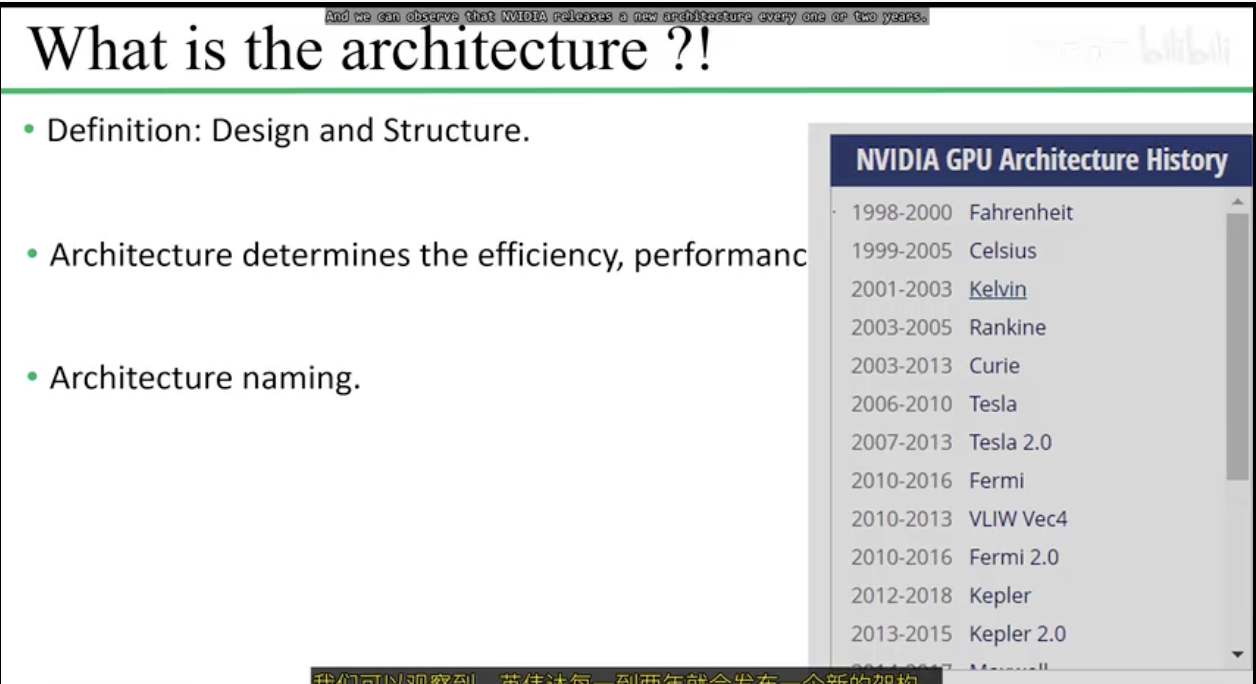
\includegraphics[width=0.75\linewidth]{resources/cuda-009.png}
    \caption{GPU架构}
    \label{fig:placeholder}
\end{figure}

接下来谈谈英伟达的不同世代。英伟达将其产品分为两个不同的类别：第一类面向普通消费者，涵盖我们在笔记本电脑、台式机和工作站
中使用的 GPU；第二类服务于高性能计算（HPC）领域，这在云计算等场景中至关重要。META、亚马逊、微软和谷歌都是 HPC 提供
商的典型代表。

第一类别包括 Tegra、GeForce 和 Quadro 等世代系列，其中 GeForce 和 Quadro 也是游戏 GPU 的热门选择——我想大多数人都
熟悉它们，因为它们常见于许多笔记本电脑中。

而第二类别（HPC 类别）中有一个世代被称为 Tesla。需要指出的是，这个 Tesla 与埃隆·马斯克的公司没有任何关联——它只是为高
性能计算设计的一系列 GPU 的统称。

\begin{figure}
    \centering
    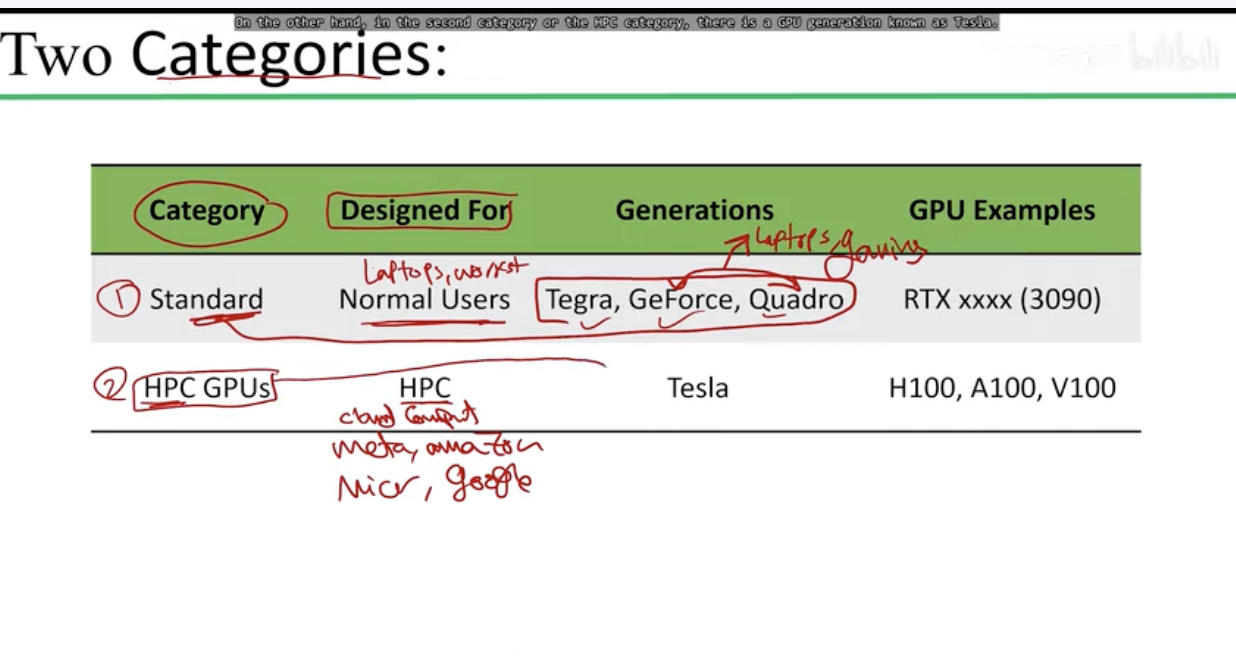
\includegraphics[width=0.75\linewidth]{resources/cuda-010.png}
    \caption{GPU架构}
    \label{fig:placeholder}
\end{figure}


\subsection{架构与世代的关系}

下表旨在总结这两个术语之间的区别：世代指的是 GPU 的具体用途，例如是用于 HPC 服务器还是标准台式机。而架构，如前所述，
指的是 GPU 芯片的设计与能力。每个架构可能包含多个不同的世代。在世代一栏，我们看到了 Tegra、GeForce、Quadro 和 Tesla 
这些名称；而 Hopper、Ampere 和 Volta 则是英伟达提供的不同架构。

\begin{figure}
    \centering
    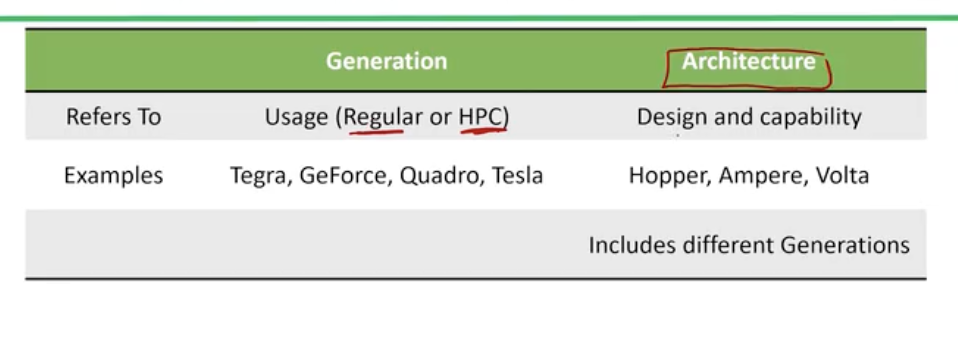
\includegraphics[width=0.75\linewidth]{resources/cuda-011.png}
    \caption{GPU架构}
    \label{fig:placeholder}
\end{figure}


为了说明这一点，考虑一下 2020 年发布的 Ampere 架构。这个架构包含了多个世代的 GPU。例如，在 Ampere 架构内，你既可以
找到 GeForce 世代的 RTX 3090，也可以找到 Tesla 世代的 A100——这两款 GPU 基于相同的 Ampere 架构芯片，但面向的应用截
然不同：RTX 3090 属于 GeForce 系列，主要设计用于游戏等消费级用途；而 A100 属于 Tesla 世代，专为超级计算机和云服务器等
HPC 环境设计。

\begin{figure}
    \centering
    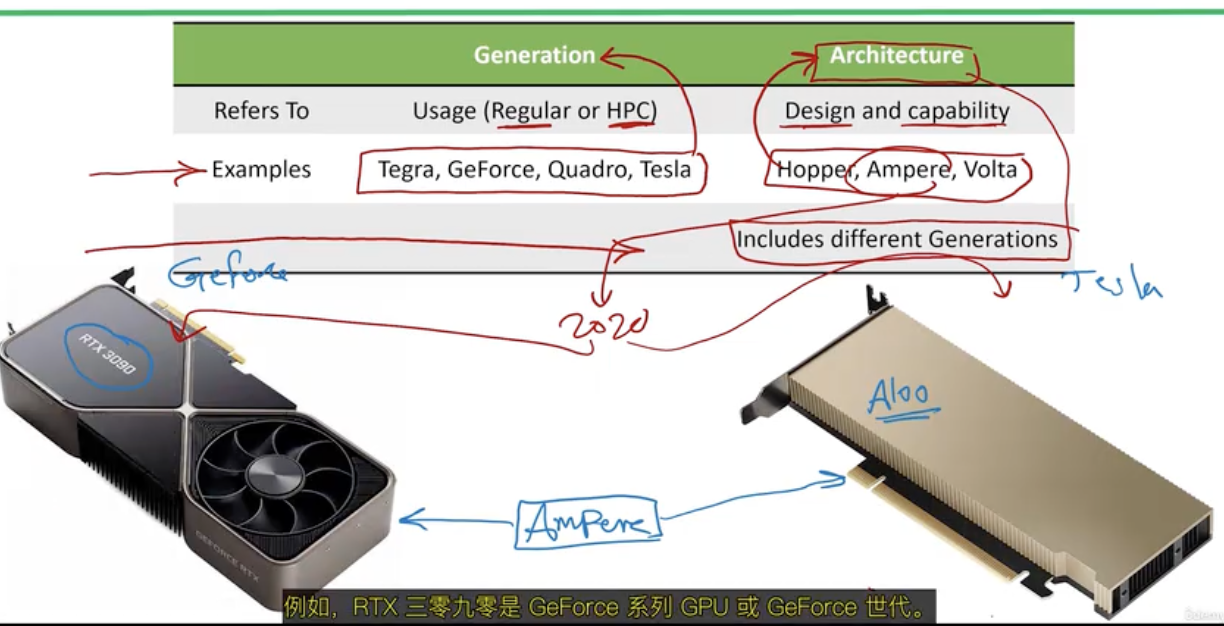
\includegraphics[width=0.75\linewidth]{resources/cuda-012.png}
    \caption{GPU架构}
    \label{fig:placeholder}
\end{figure}


总之，我们可以这样理解：每当英伟达整合了新的软件或硬件增强功能，就会宣布一个新架构；然后基于这个新架构，再为普通消费者和
HPC 领域分别开发不同世代的 GPU。

\subsection{GPU世代分类}

现在让我们深入探讨不同类型的世代。下表展示了英伟达最知名的 GPU 世代之间的区别：Tegra、GeForce、Quadro 和 Tesla。

首先来看 Tegra。Tegra 是英伟达为智能手机、平板电脑和移动互联网设备等移动平台开发的片上系统（SoC），将 GPU 和 CPU 集成
在单一芯片中。第一款使用 Tegra 的产品是微软的 Zune HD 媒体播放器，于 2009 年 9 月发布。2017 年 3 月 15 日，Tech 
Insights 披露了任天堂 Switch，它同样由 Tegra 芯片驱动。

\begin{figure}
    \centering
    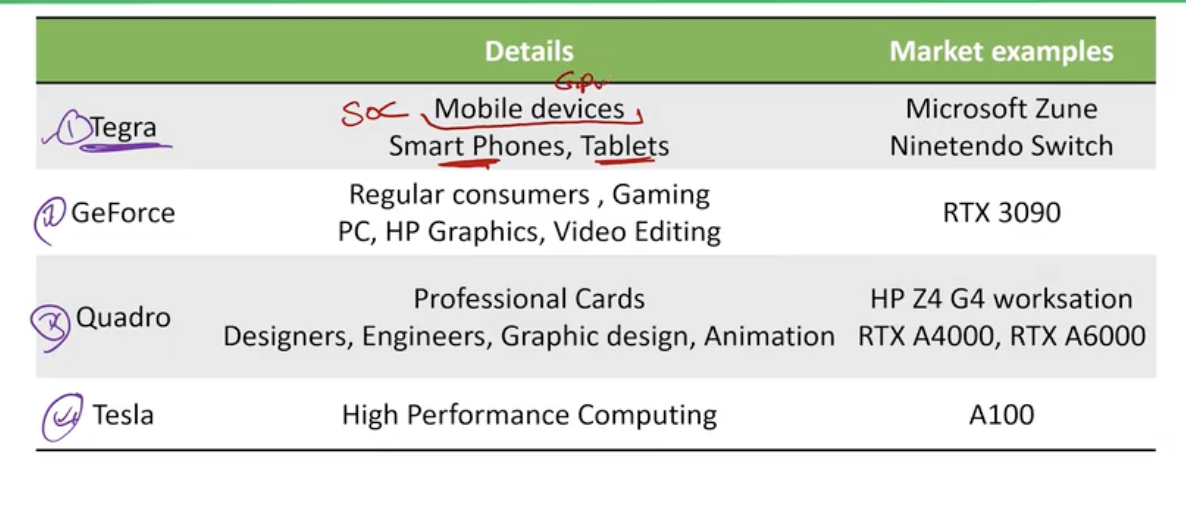
\includegraphics[width=0.75\linewidth]{resources/cuda-013.png}
    \caption{GPU架构}
    \label{fig:placeholder}
\end{figure}


接下来是 GeForce GPU——请注意，这一世代的 GPU 专为个人计算机打造，面向消费级市场，尤其是游戏玩家。这里说的是三维图形渲染
和游戏中的高性能，而非 HPC 级别的计算。它们也被普通消费者用于视频编辑和其他图形密集型任务。GeForce 系列中一个突出的例
子是 RTX 系列，如 GeForce RTX 3090、3080、3070 和 3060，这些是当前市场上该世代最知名的 GPU。接下来是 Quadro GPU——专业工作站显卡，专为需要高精度和计算能力的设计师和工程师打造。Quadro GPU 经过优化，适用于高级图
形设计、视频编辑和动画等专业软件。它在许多笔记本电脑中广泛使用，以提供增强的性能。此外，最新工作站（如 HP Z 系列）通常
也使用 Quadro GPU。

在离开 Quadro GPU 这个话题之前，让我们花点时间讨论一些最近的更新。例如 HP 最近推出的一款工作站——HP Z4 G4，这款工
作站可以配备高端的英伟达 Quadro RTX 显卡。但在未来的 GPU 中，我们将不再看到 Quadro 品牌。正如下图所示（来源见链接所
示），Quadro 命名已被 RTX 标签取代，我们只会看到 RTX 标签。

此外，同一网页包含一个表格，展示了各种 Quadro 系列与其对应英伟达架构之间的关系，以及它们在 RTX 系列中的新命名等价物。
表格的排列方式为：第一列列出了不同的 Quadro 系列，如 8000 和 6000 等。以 6000 系列为例，这一行展示了不同架构下的命名惯
例——在 Maxwell 架构中前缀是 M，在 Pascal 架构中前缀是 P，命名惯例为 Quadro 后跟系列数字（如 6000），前面加上架构的首字母。

\begin{figure}
    \centering
    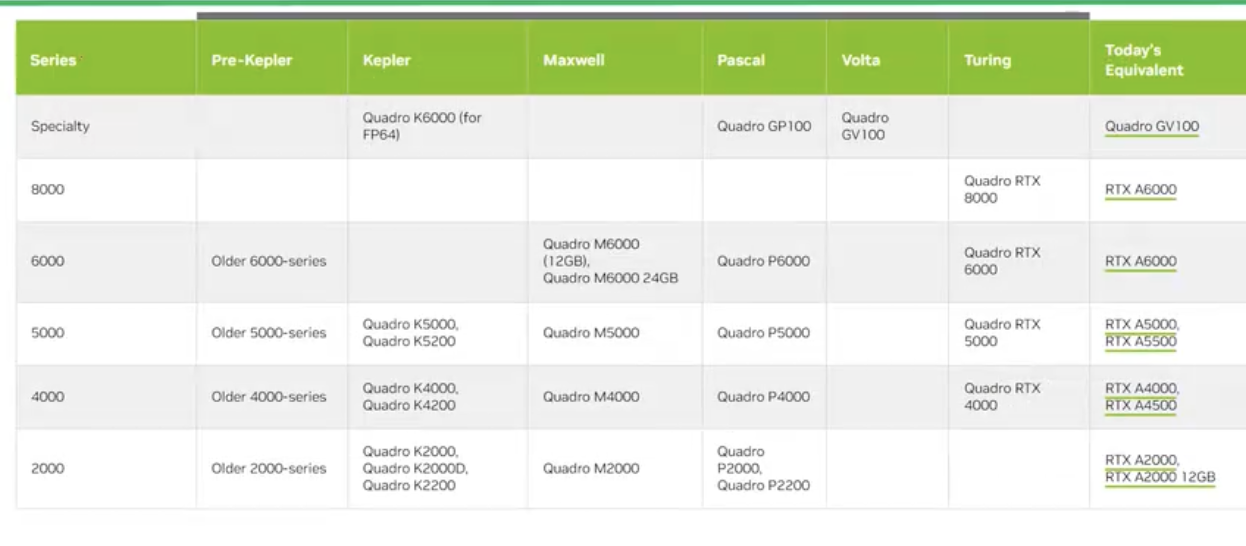
\includegraphics[width=0.75\linewidth]{resources/cuda-014.png}
    \caption{GPU架构}
    \label{fig:placeholder}
\end{figure}


在 Pascal 中前缀是 P。但在 Turing 架构中，RTX 标签被插入在 Quadro 和系列数字之间。正如我们所见，如果你打算在并行编
程或 GPU 领域工作，了解 GPU 的命名规则非常重要。然而，从 Ampere 架构开始，英伟达已经弃用了 Quadro 品牌，只使用 RTX 
前缀。

还有一点需要注意：在弃用 Quadro 术语之前，英伟达将 RTX 名称同时用于 Quadro 和 GeForce 两条产品线。例如 RTX 30XX 系
列，包括 RTX 3090、3080、3070 和 3060 等型号，都属于面向消费者（尤其是游戏玩家）的 GeForce 家族。

在专业领域（如设计和内容创作），正如表格所描绘的，曾存在 Quadro RTX 这样的型号。我们有 GeForce RTX 和 Quadro RTX 两
个系列，例如 Quadro RTX 4000、Quadro RTX 5000 和 Quadro RTX 8000。RTX 标签同时出现在 GeForce 世代和 Quadro 世代
中。但需要记住的是，在未来的 GPU 中，我们将不再看到 Quadro 品牌，只会看到 RTX。虽然这些信息乍一看可能让人应接不暇，但
这完全正常——当你更深入地研究 GPU 行业并开始使用这些产品时，命名和术语会变得更加熟悉，也更容易理解。

总而言之，我们在最顶层有 GPU 架构，每个架构可用于生产不同的世代。


\subsection{GeForce与Tesla在超级计算机中的应用}

现在让我们来看两种来自不同世代的 GPU 的真实案例，每个世代针对不同的市场细分——从 GeForce 这样的普通消费级 GPU 到为 HPC
设计的 Tesla 系列。正是这种区别，使得在全球前 500 名超级计算机中看到 GeForce 系列的 GPU 相当罕见，因为它并非为超级计算
机设计，而是为普通台式机和工作站设计的。

让我们深入 TOP500 网站进一步探索。如下所示，这是当年六月发布的前 500 名超级计算机列表。如果我们搜索 A100、V100 和
P100 等 GPU——这些都属于 Tesla 世代——可以观察到许多超级计算机采用了它们，因为 Tesla 正是为超级计算机等用途设计的。我
们将在接下来的章节中详细而深入地讨论这些 GPU。

另一方面，如果我们搜索 RTX 系列，结果显示在排名靠前的超级计算机中没有此类应用。我想现在你已经清楚了 GeForce 与 Tesla 
世代之间的区别。理解所有这些区别对于为你的特定应用选择正确的 GPU 至关重要。我们将在接下来的章节中更深入地介绍 GeForce 
和 Tesla 等不同世代。
